\chapter{Simulation Study Design and Methods}
\label{C:chap_sim_design}


To analyse the performance of the different methods described in Chapter \ref{CHAP:methods} simulations of clinical trials was performed. This chapter describes the overall framework used and the rationale for the choice of parameters kept fixed and those modified by scenario. Some aspects are inspired by choices made in the simulation study reported in \cite{Morden2011}.

\section{Simulation framework}

\label{section:studydesign}

\subsection{Entry and exit times}
Similar to \cite{Morden2011} a uniform distribution was assumed for entry to the study. However, to increase the amount of censoring observed enrolment was assumed to occur over a two year period with all patients censored at 3 years after the study start meaning all patients were followed for between 1 and 3 years.

\subsection{Underlying Survival Times}
Following \cite{Morden2011} a sample size of 500 patients per dataset was chosen with 250 allocated to control and experimental treatment. For all 500 patients the baseline Time to Progression (TTP) and Overall Survival (OS) were generated from a weibull distribution with survival function as shown in Equation \ref{E:chap_simdesign:weibull}. For Time to Progression the parameters chosen were $\gamma_{TTP}=1.5$ and $\lambda_{TTP}=2$, for overall survival the parameters were $\gamma_{OS}=1.2$ and $\lambda_{OS}=0.3$. From these two survival times a progression free survival (PFS) time is defined as the minimum of time to progression (TTP) and overall survival (OS). It can be seen in Figure \ref{F:chap_sim_design:exampleKM} that these parameters result in realistic survival curves compared to those seen in e.g.  \cite{EMILIA}.

\begin{equation}
\label{E:chap_simdesign:weibull}
S(t) = \exp(-\lambda t^\gamma)
\end{equation}

\subsubsection{Correlation between TTP and OS}
\label{S:chap_sim_design:corr}
As discussed in Section \ref{S:chap_intro:correlation} the main focus of this dissertation is to investigate the impact of correlation between TTP and OS so on a patient level these are forced to be correlated with a known correlation (denoted $\rho$). When selecting the range of $\rho$ to investigate Table \ref{T:chap_intro:corr} was consulted, however, this mostly reports the correlation between PFS (a composite of TTP and OS) with OS. As PFS is a composite of TTP and OS it shows a some correlation with OS even when TTP is and OS is uncorrelated as illustrated in Figure \ref{F:chap_sim_design:corr1}.
\begin{figure}[h!]
\centering
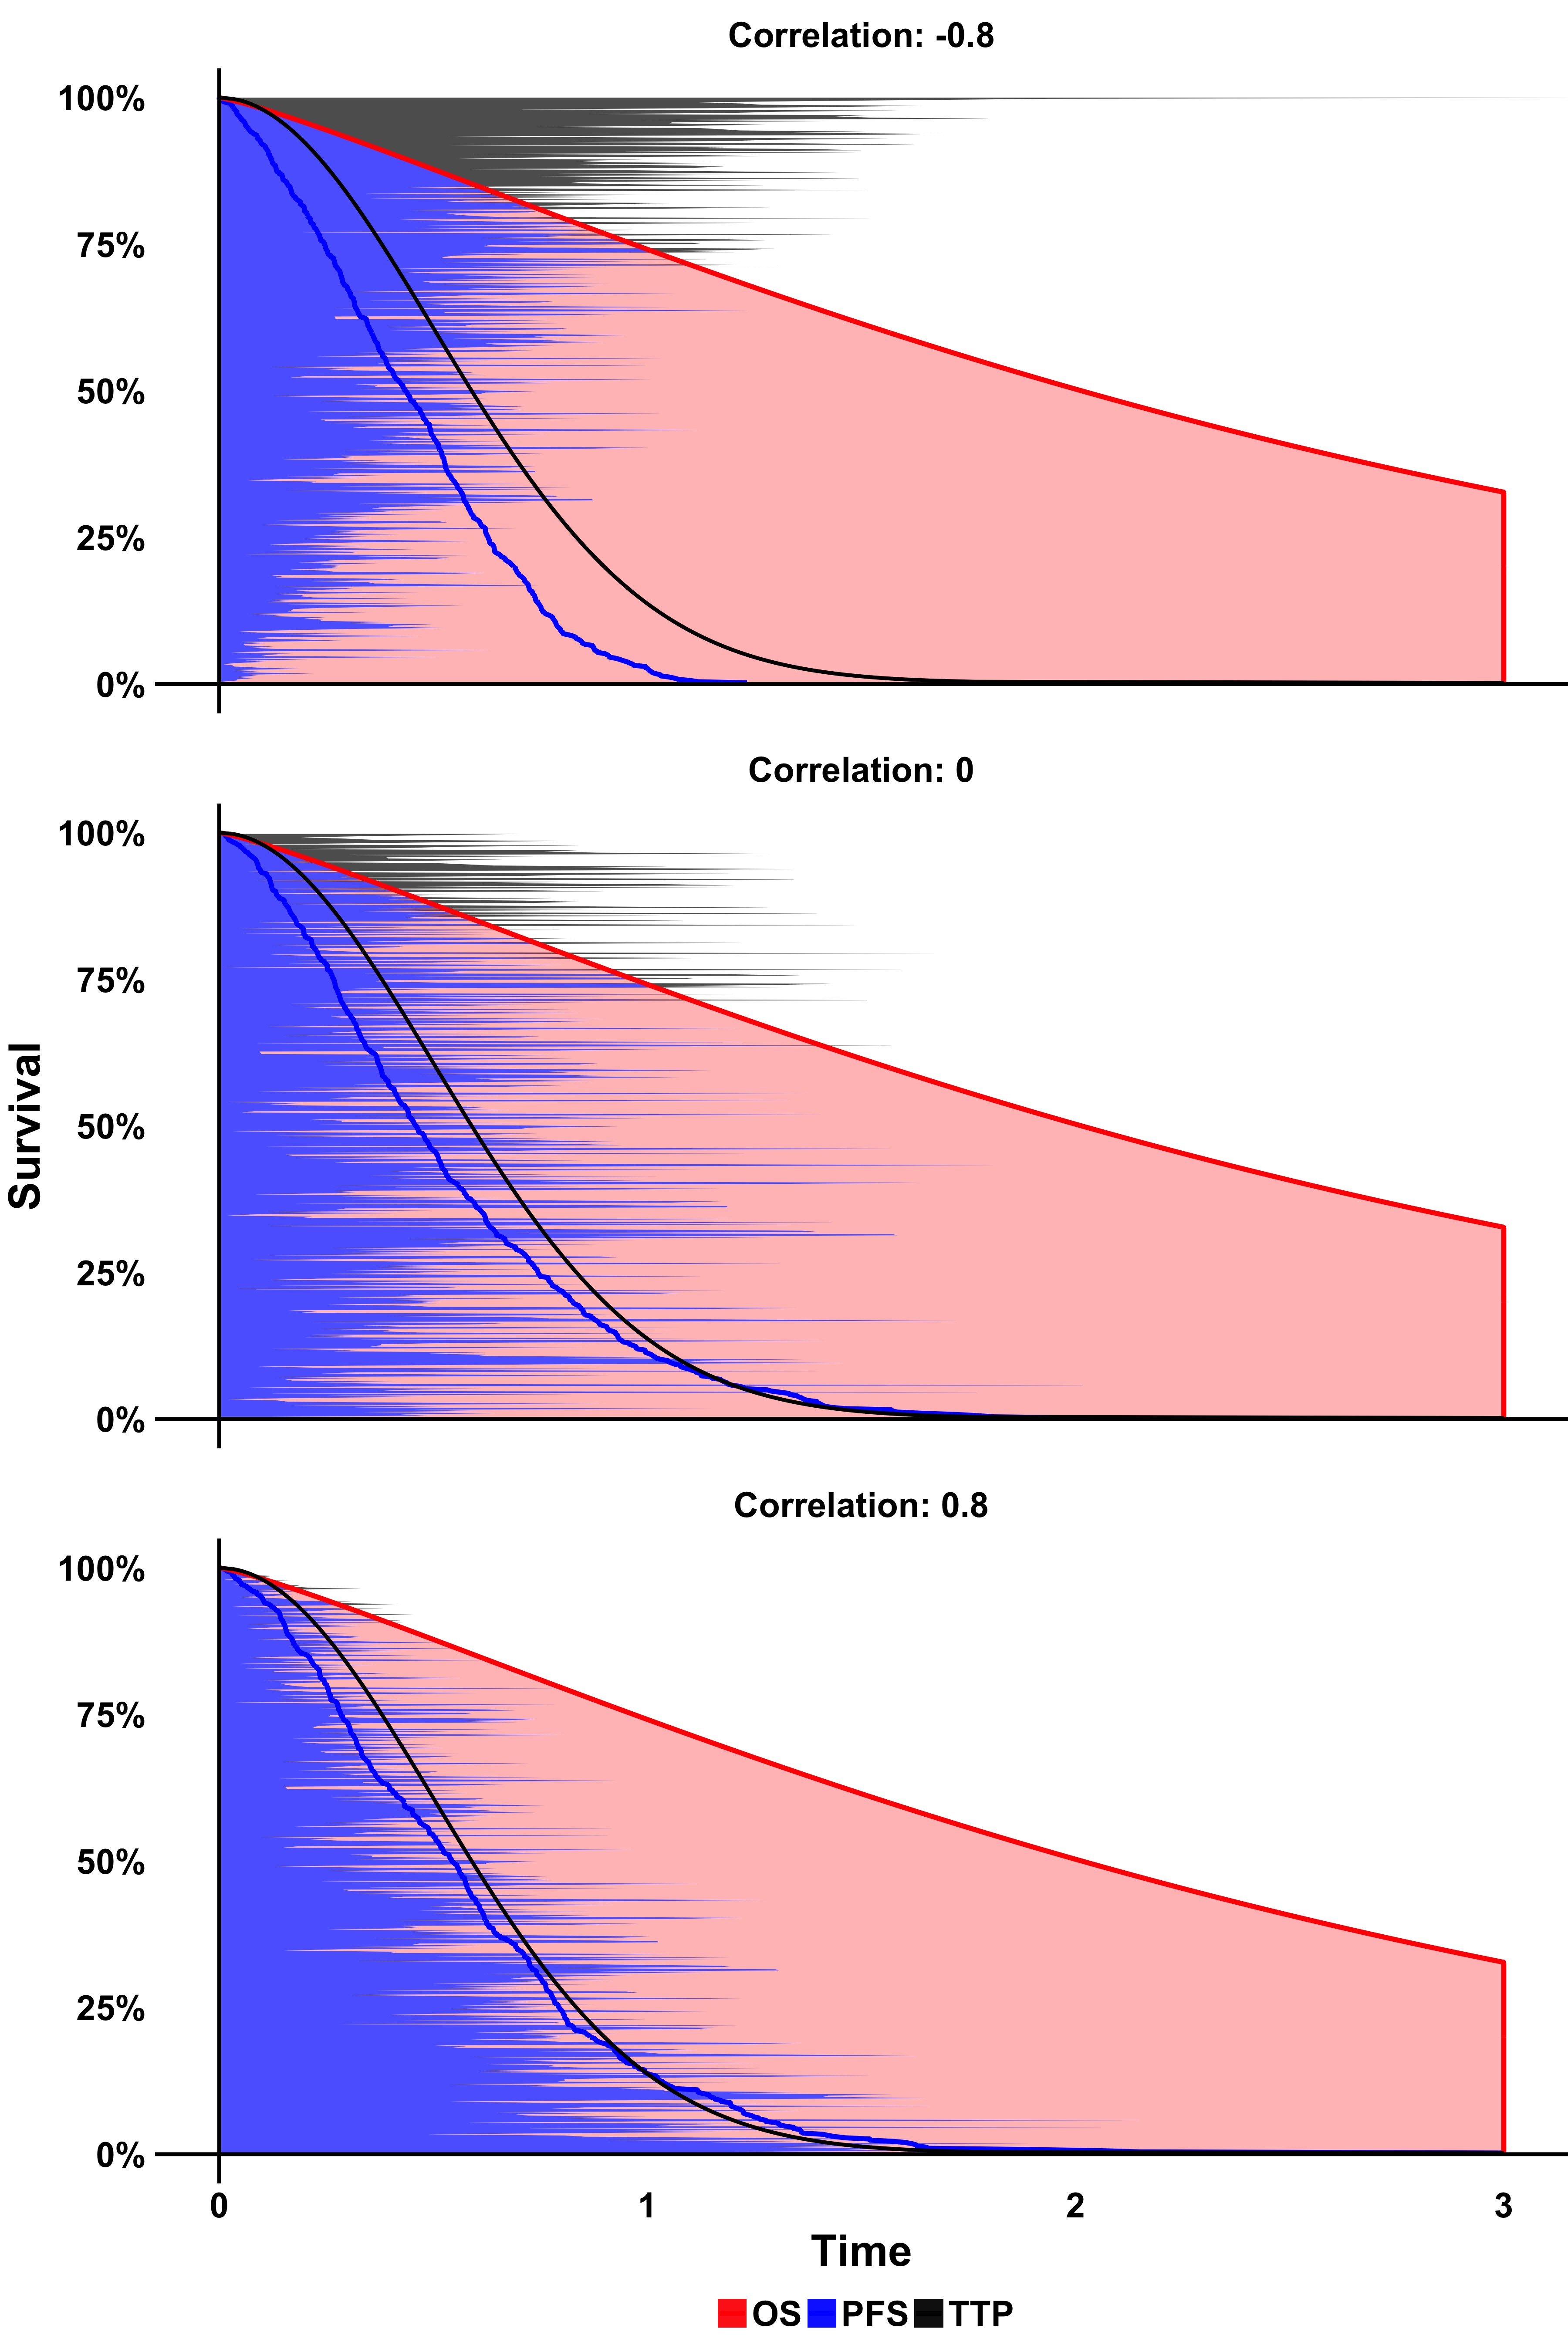
\includegraphics[width=10cm]{images/chap_simdesign/sim1corr.png}
\caption{\label{F:chap_sim_design:corr1}
An illustration of the time to progression (TTP), progression free survival (PFS) and overall survival times for strong negative, none and strong positive correlations between TTP and OS. The filled area shows the PFS and TTP by patient associated with OS. For strong negative correlation it can be seen that the TTP is often longer than OS meaning PFS is often OS in this case. For strong positive correlation it can be seen that longer TTP is associated with longer OS. With no correlation TTP is not related to OS, however, as PFS is a composite of OS and TTP it still shows some correlation with OS.} 
\end{figure}

To investigate what the resulting correlation between PFS and OS is for the simulations here the simplest method described in \cite{Buyse2007} was used. That is the correlation between the Kaplan-Meier estimates of PFS at 6 months and OS at 12 months were estimated from simulated trial data for candidate values of $\rho$ between 0 and 1 for 200 simulated trials each. The results of this are shown in Figure \ref{F:chap_sim_design:pfs_corr}. Based on this while a range of correlation between TTP and OS between 0 and 1 will be investigated a correlation of between 0.4 and 0.8 for TTP and OS seems to yield the most plausible correlations between PFS and OS.

\clearpage

\begin{figure}[h!]
\centering
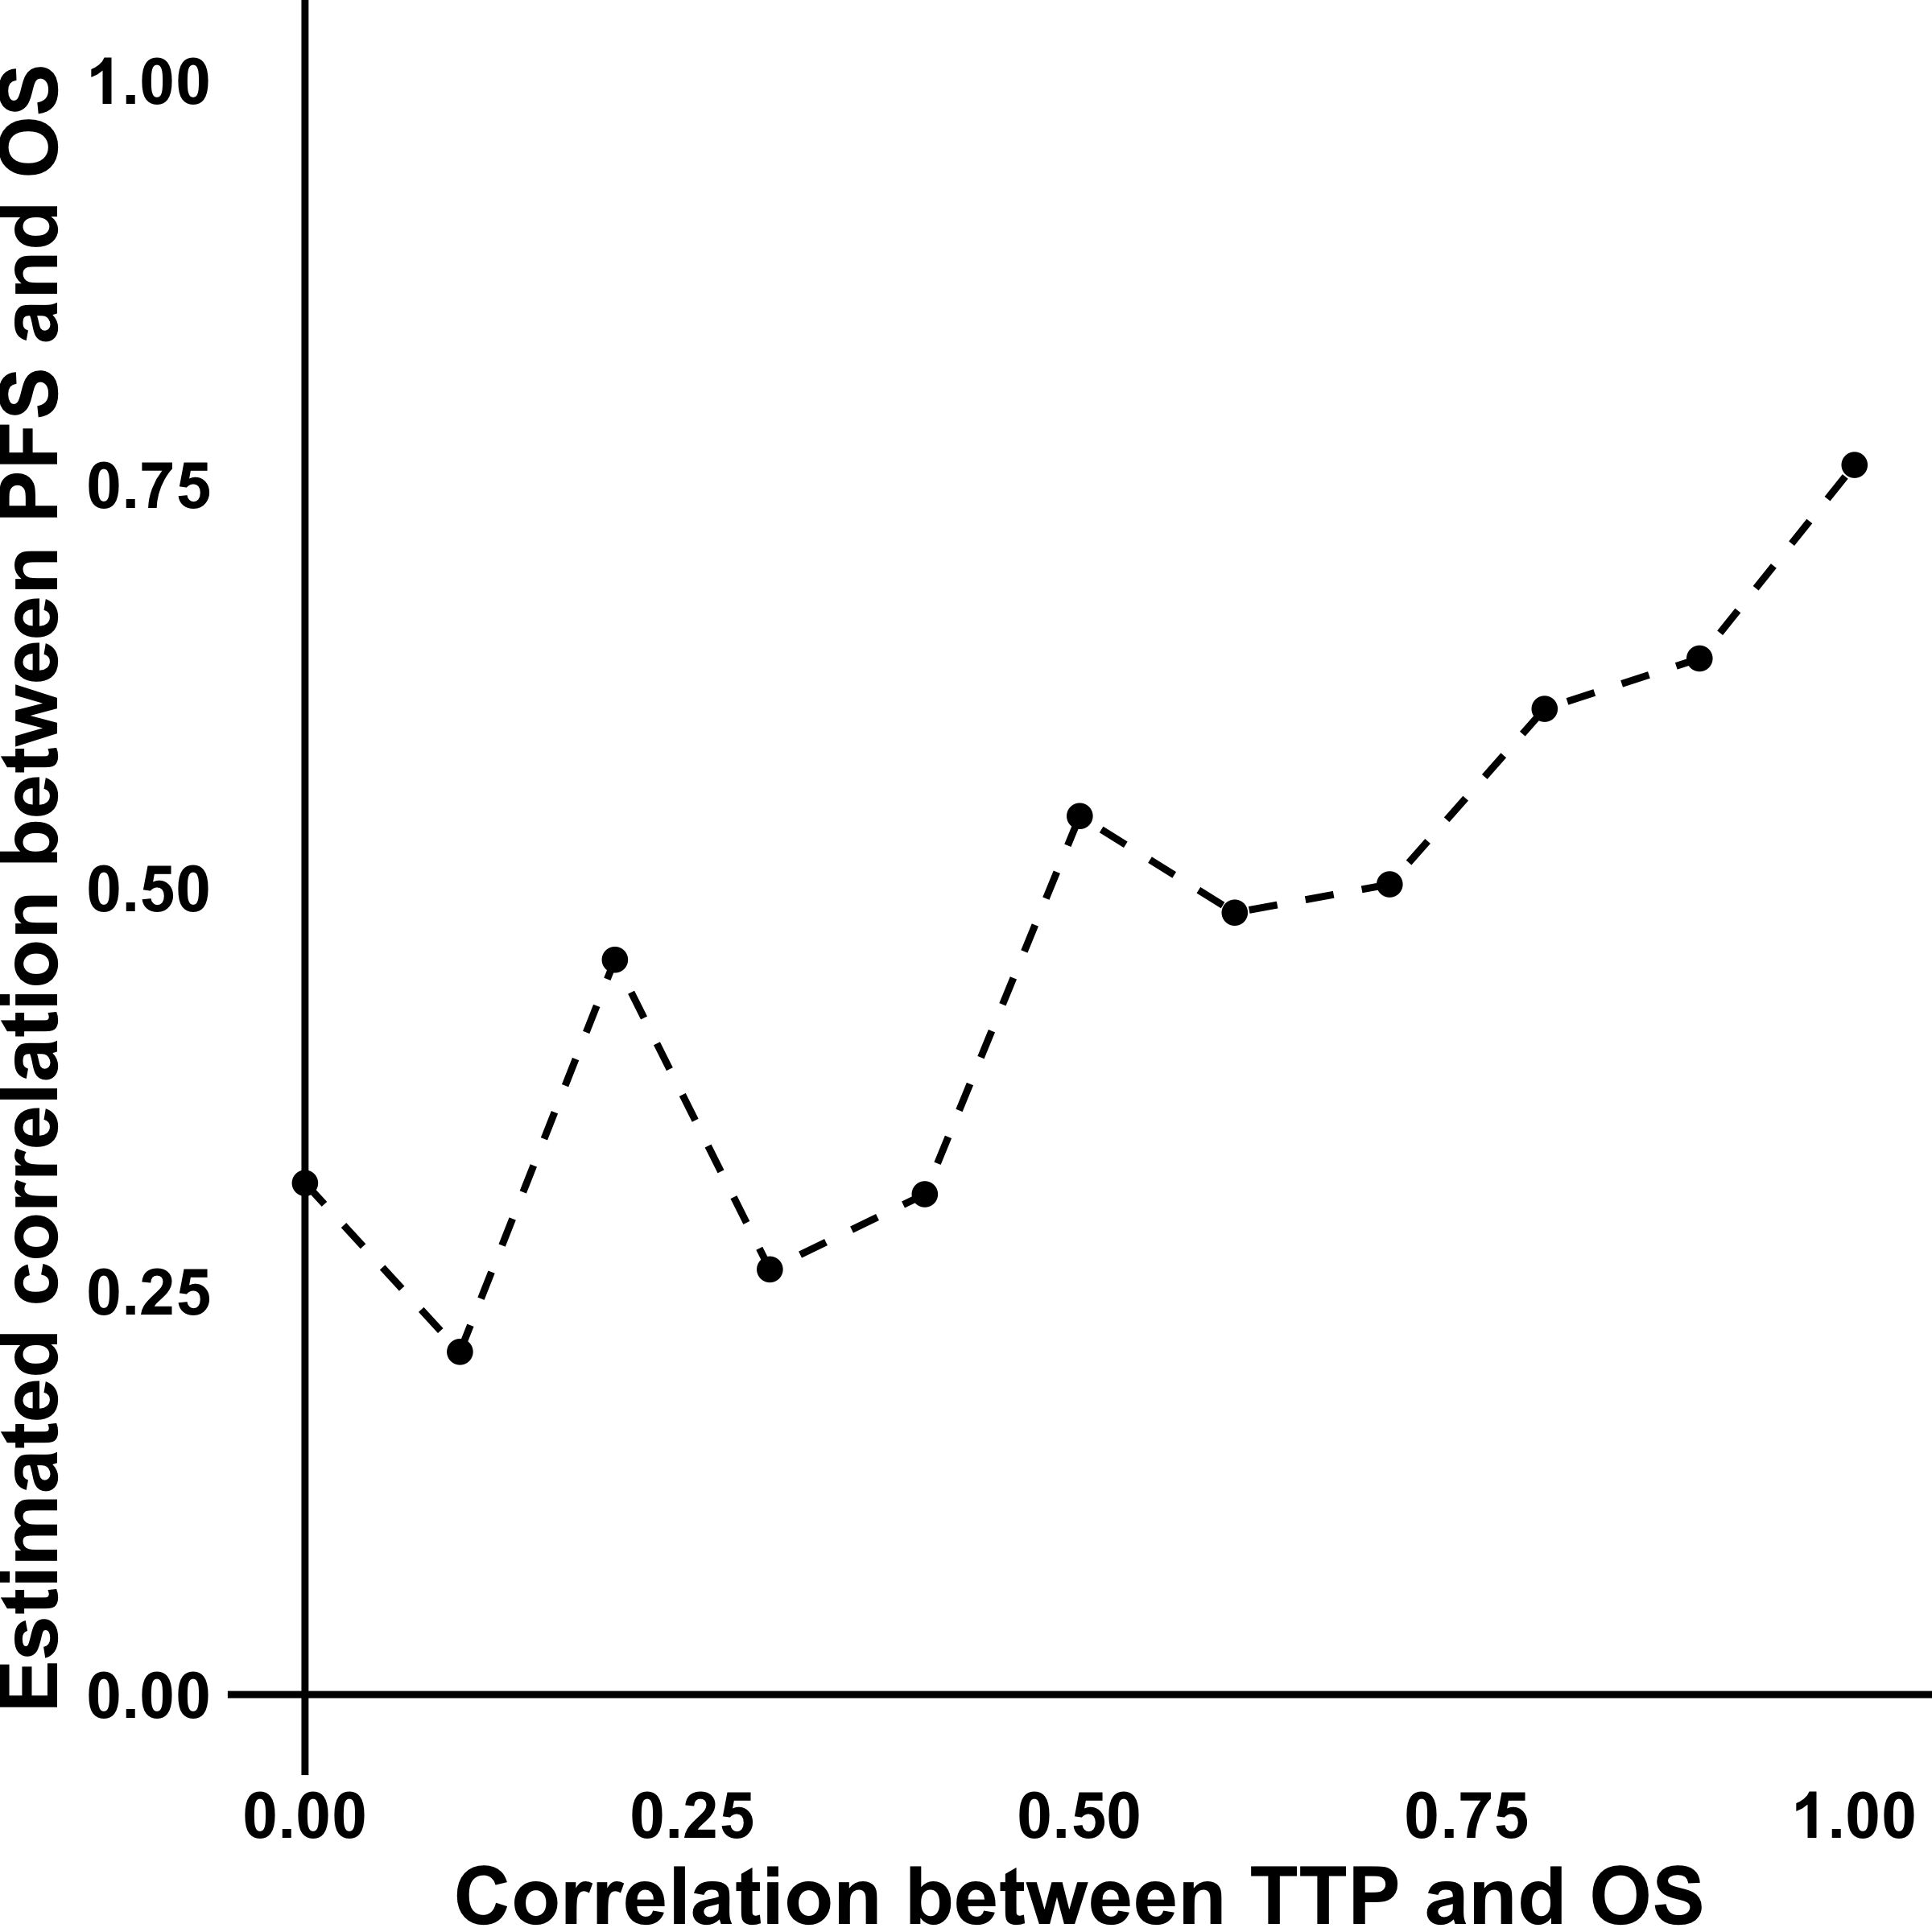
\includegraphics[width=8cm]{images/chap_simdesign/PFSOScor.png}
\caption{\label{F:chap_sim_design:pfs_corr} Estimates for the relationship between correlation in progression free survival (PFS) and OS for a range of correlations between time to progression (TTP) and overall survival (OS) using the underlying survival times.} 
\end{figure}


\subsection{Switching mechanism}
\label{S:chap_sim_design:switchmec}
As discussed in \ref{S:chap_intro:pattern} different patterns of switching may exist including restrictions on a patient and on a study level. For simplicity of simulation I am only going to consider that patients can switch at the time of progression (denoted $T_{PD}$). However, this still leaves the question of when in the study patients are allowed to switch. To control this I consider a proportion of PFS events that must occur before switching is allowed with only patients who progress after this time point being allowed to switch. When this required proportion is 0 this represents the scenario of switching being pre-planned from day 1 and otherwise it represents a scenario where switching is introduced after an interim analysis or external event.

For each simulation a target proportion of control patients who will switch to experimental therapy is defined. As only patients who progress after the defined number of PFS events occur and who have PFS less than OS and also less than follow-up time can be observed to switch this group is defined as the switch eligible population. From this switch eligible population a random selection is made so the target proportion of the control arm switches.

\subsubsection{Implications for prognosis of switch population}
Given the way survival times are generated when there is a strong positive correlation between time to progression (TTP) and overall survival (OS) the switch eligible population will contain more patients with a poor prognosis (in terms of overall survival). This is because patients with a good prognosis will have a longer time to progression and will be excluded from the switch eligible population as their progression free survival time is more likely to  extend beyond the follow up time.

\subsection{Prognostic covariates}

With all simulation studies a balance has to be made between realistically capturing the underlying problem and having a tractable problem. As discussed in the previous section introducing a correlation between TTP and OS in itself generates differential prognosis of switchers versus non-switchers given the constraints on who can be observed to switch within the study follow-up time. For this reason I choose not not to implement any additional prognostic covariates and focus instead just on the impact of correlation. 

\clearpage

\subsection{Adjusting survival times for treatment received}
\label{S:chap_sim_design:trtEffects}

For all scenarios a relatively large treatment effect on time to progression is considered. This is applied as a reduction in the hazard of progression defined as a log hazard ratio ($\beta_{pd}$) and will be constant at $\log(0.4)$ in all simulations. For all scenarios time on treatment for all patients will be fixed as time until progression i.e. it is simulated that no patients discontinue early or for any reason other than progression. For switch patients no time to second progression will be simulated but for simplicity the time on switch treatment will be taken as as the time to first progression (including the treatment effect on progression). The treatment effect on overall survival is then applied as four separate time dependent covariates representing an effect while on treatment i.e. until PD denoted $\beta_{1a}$, an effect after PD given prior treatment $\beta_{1b}$, an effect on switch treatment while on switch treatment denoted $\beta_2a$ and an effect after discontinuing switch treatment denoted $\beta_2b$. These four treatment effects are illustrated in Figure \ref{F:chap_sim_design:trtEffects}. 

\begin{figure}[h!]
\centering
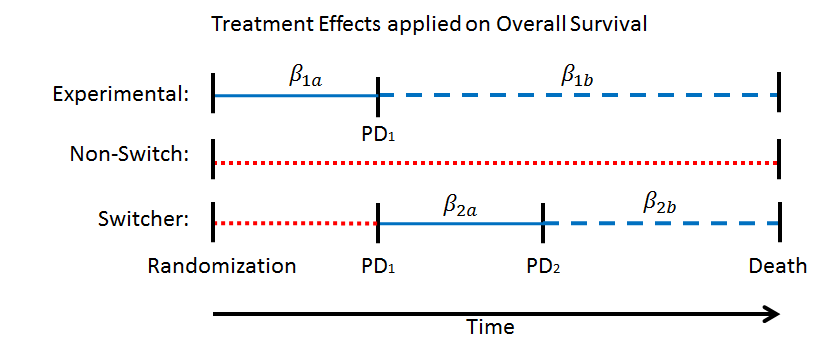
\includegraphics[width=12cm]{images/chap_simdesign/simTrtEff.png}
\caption{\label{F:chap_sim_design:trtEffects} An illustration of how the time varying treatment effects $\beta_{1a}$, $\beta_{1b}$, $\beta_{2a}$ and $\beta_{2b}$ apply to a patient randomized to the experimental arm, a non-switch patient and a switch patient. $PD_{1}$ denotes the first progression while $PD_2$ denotes the second progression after initiation of switch treatment. For simplicity only a single time to progression is simulated and assumed to apply for first and second progression.}
\end{figure}

\clearpage

\subsection{Summary of simulation parameters}

Table \ref{T:chap_sim_design:parms} shows the parameters that can be varied within this simulation framework and indicates those that are fixed across all scenarios and those which are varied across different scenarios. An illustration of the survival curves generated for two example scenarios are shown in Figure \ref{F:chap_sim_design:exampleKM}. The scenarios shown are where there is a moderate treatment effect that applies at all times ($\beta_{1a}=\beta_{1b}=\beta_{2a}=\beta_{2b}=\log(0.7)$) and a scenario where treatment reduces the risk of treatment during treatment only and has no effect afterwards ($\beta_{1a}=\beta_{2a}=\log(0.01)$ and $\beta_{1b}=\beta_{2b}=\log(1)$). 


\begin{table}[ht] 
\caption{Summary of simulation parameters}
\centering 
\begin{tabular}{ l l r}
\hline
\hline
Parameter & \multicolumn{2}{l}{Description}  \\
\hline
$\rho$    & \multicolumn{2}{l}{Correlation between TTP and OS} \\
$T_{\verb+switch+}$ & \multicolumn{2}{l}{\% patients experiencing PFS event before switch allowed}  \\
$p_{\verb+SWITCH+}$ & \multicolumn{2}{l}{Proportion of control arm who switch} \\
$\exp(\beta_{1a})$ & \multicolumn{2}{l}{Hazard ratio for OS during randomized treatment} \\  
$\exp(\beta_{1b})$ & \multicolumn{2}{l}{Hazard ratio following randomized treatment}     \\
$\exp(\beta_{2a})$ & \multicolumn{2}{l}{Hazard ratio for OS during switch treatment}     \\  
$\exp(\beta_{2b})$ & \multicolumn{2}{l}{Hazard ratio for OS following switch treatment}  \\
\hline
\multicolumn{3}{c}{Parameters held fixed across all scenarios} \\
Parameter & Description & Value  \\
\hline 
$N$ & Number of patients (with 1:1 randomization) & $500$  \\
$\exp(\beta_{pd})$ & Hazard Ratio for TTP & $0.4$  \\
$\lambda_{TTP}$ & Scale for TTP weibull baseline hazard & $2$     \\ 
$\gamma_{TTP}$  & Shape for TTP weibull baseline hazard & $1.5$  \\
$\lambda_{OS}$ & Scale for OS weibull baseline hazard  & $0.3$   \\ 
$\gamma_{TTP}$ & Shape for OS weibull baseline hazard & $1.2$   \\
\hline
\end{tabular} 
\label{T:chap_sim_design:parms}
\end{table}


\begin{figure}[h!]
\centering
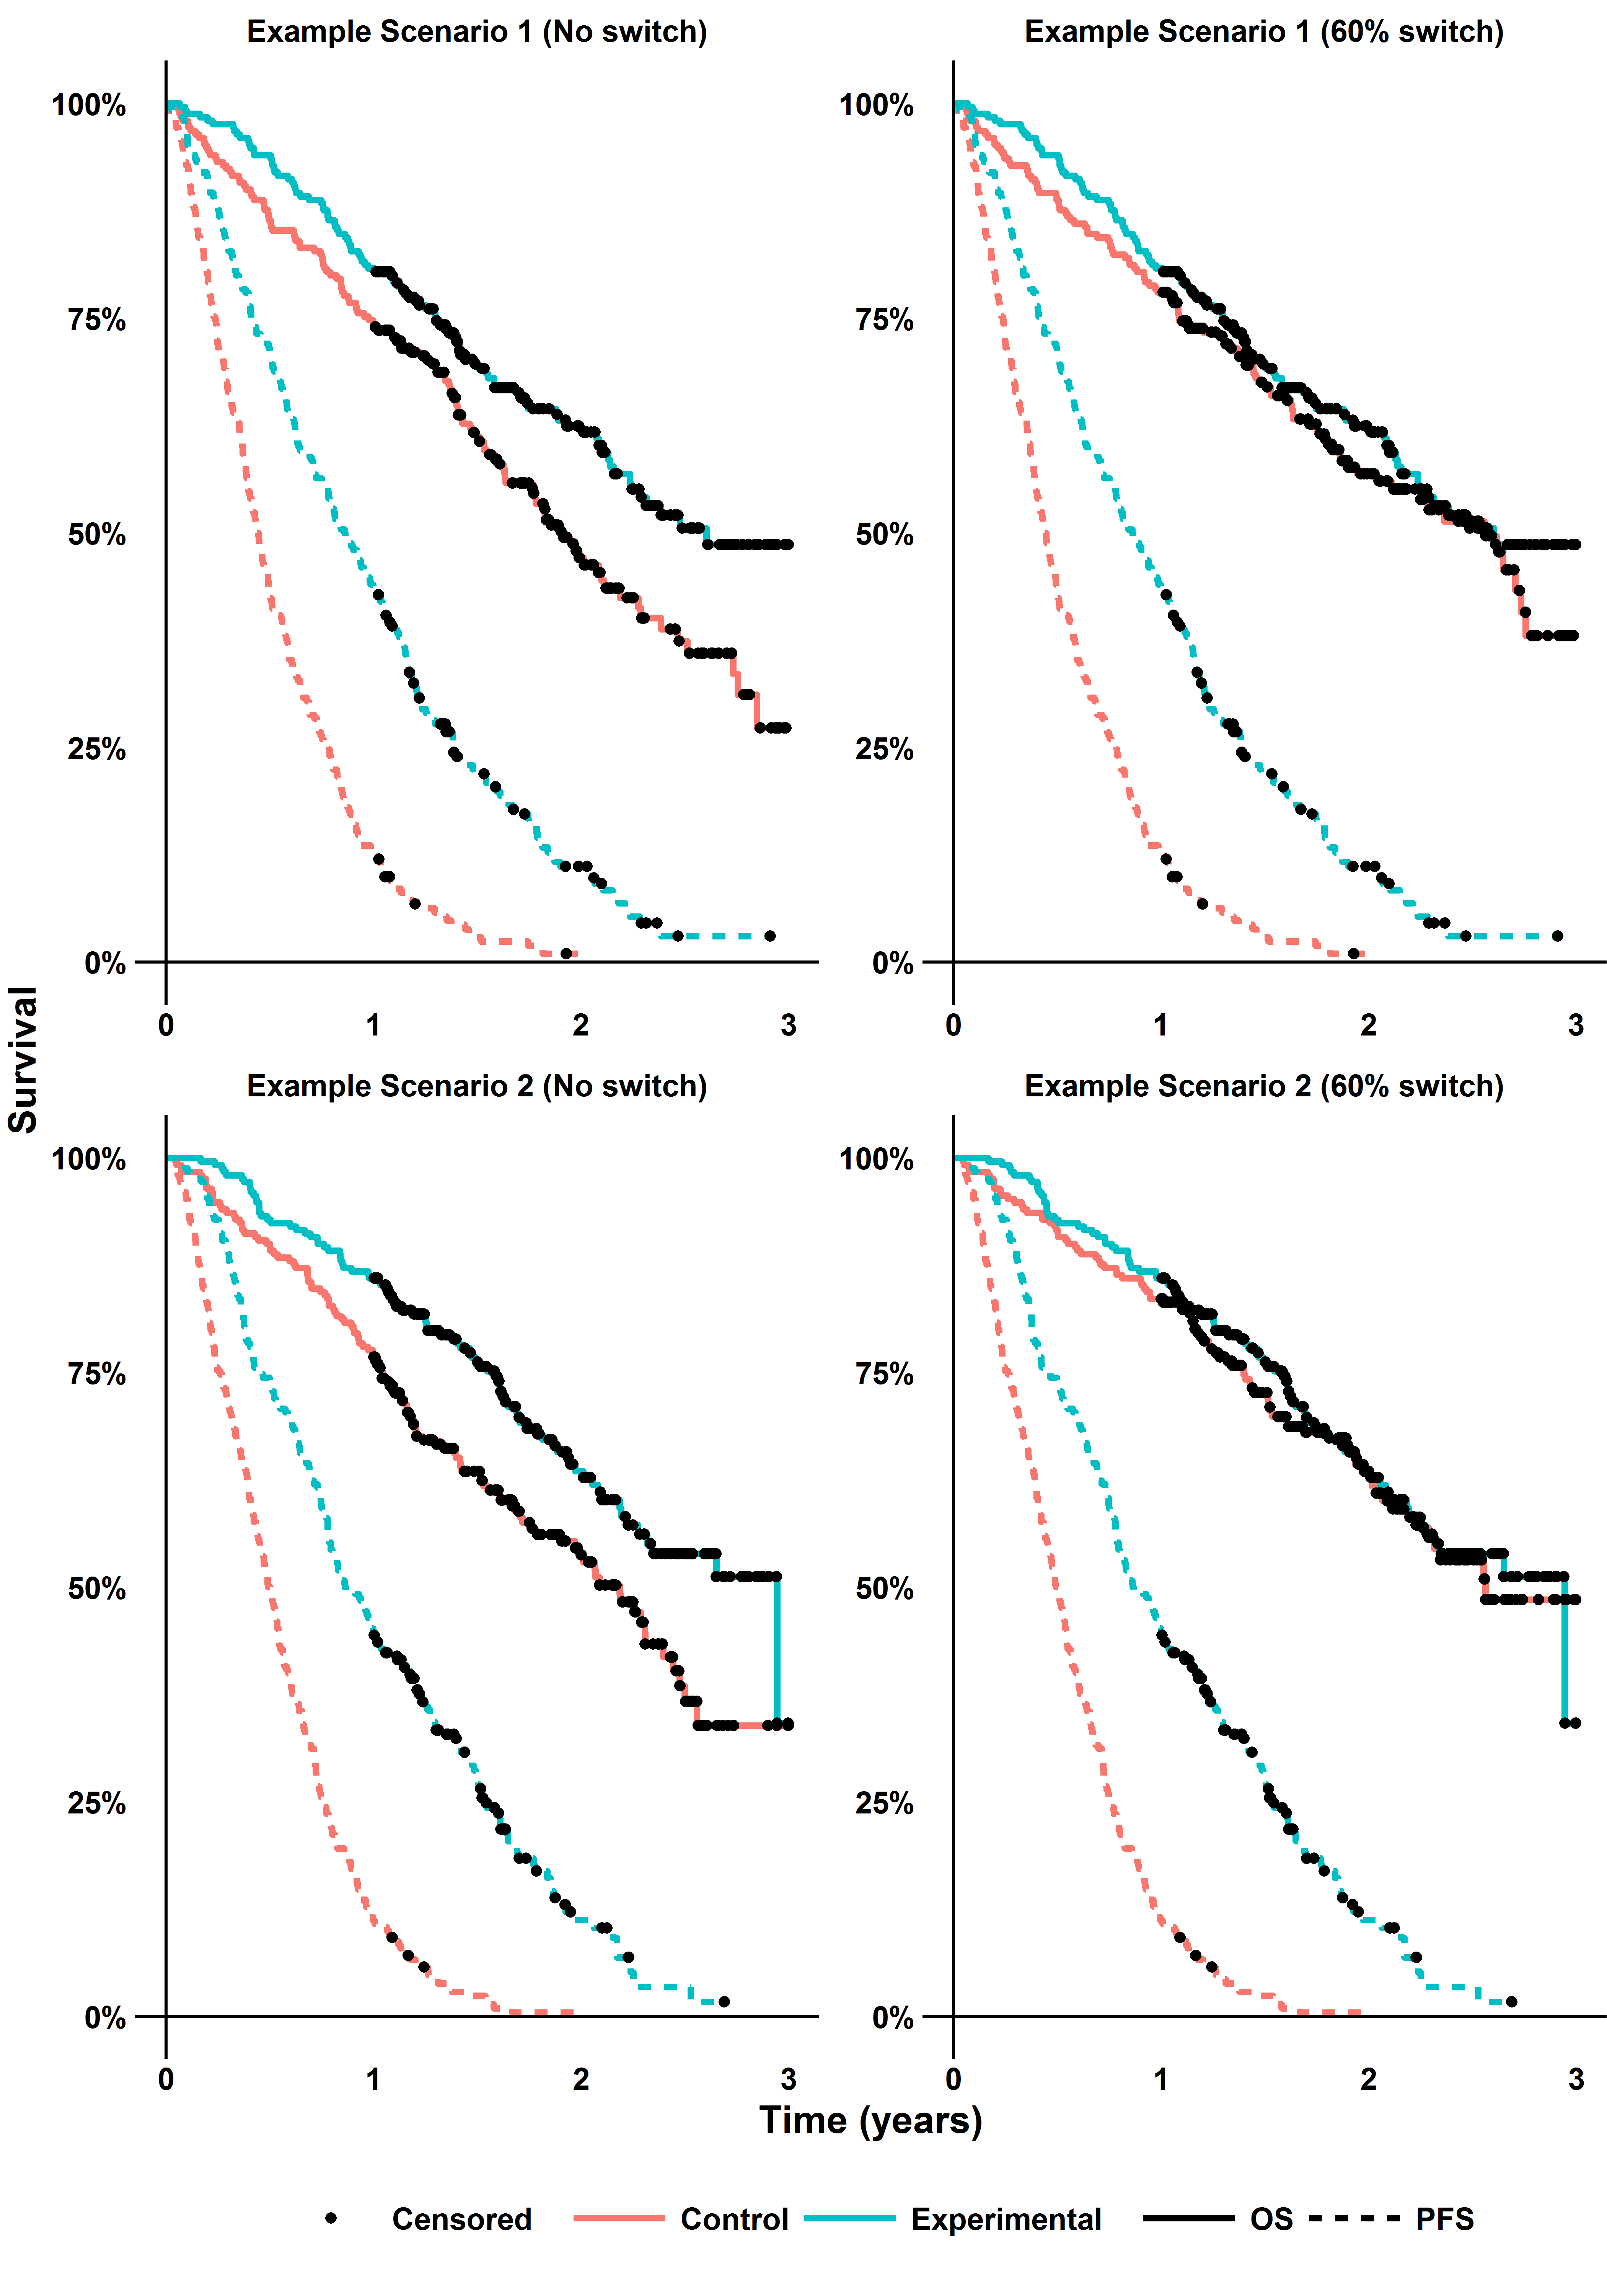
\includegraphics[width=12cm]{images/chap_simdesign/examplekm.png}
\caption{\label{F:chap_sim_design:exampleKM} The resulting survival curves for the simulation framework described in this chapter. Both example scenarios have $\rho=0.6$ and switching allowed from randomization. The treatment effects for Example Scenario 1 are $\beta_{1a} = \beta_{1b} = \beta_{2a} = \beta_{2b} = \log(0.7)$, that is a hazard ratio for experimental treatment in randomized or switch use of $0.7$. For Example Scenario 2 $\beta_{1a} = \beta_{2a} = \log(0.01)$ and $\beta_{1b}=\beta_{2a}=\log(1)$ meaning treatment only reduces the risk of death during progression free survival. While a hazard ratio of $0.01$ during treatment may seem large it is consistent with an approximate average hazard ratio for treatment of $0.65$ for a comparison of the arms as randomized.
}
\end{figure}

\clearpage


\section{Method to simulate correlated survival times incorporating treatment effect}
\label{S:chap_sim_design:simsurv}
In general if one can define the inverse of the cumulative distribution function $F^{-1}(p), p\in [0,1]$ it is possible to simulate random numbers following an arbitrary distribution through generating uniform random numbers. For survival data \cite{Bender2005} note that if the inverse of the cumulative hazard function $H(t)$ can be evaluated this can also be used as $F^{-1}(p) = H^{-1}(-log(p))$. This approach is modified to enable two correlated survival times to be generated with correlation $\rho$ as follows: 
\begin{enumerate}
\item Generate two independent standard normal random variables $X_0, X_1$ 
\item Define $X_2 = \rho X_1 + \sqrt{1-\rho^2} X_0 $ so $X_1$ and $X_2$ are correlated standard normal random variables
\item Define $U_i = \phi (X_i), i=1,2$ so $U_1$ and $U_2$ are correlated uniform random variables
\item Define $T_i = H_i^{-1}(-log(U_i)), i=1,2$ where $H_1^{-1}(t)$ and $H_2^{-1}(t)$ are inverse hazard functions so $T_1$ and $T_2$ are correlated survival times.
\end{enumerate}

Therefore to generate the correlated time to progression (TTP) and overall survival (OS) times required by this simulation framework it is just necessary to derive the inverse hazard function for TTP and OS.

\subsection{Simulating Time to Progression (TTP)}

The hazard function including a treatment effect on progression can easily be written as shown in Equation \ref{E:chap_sim_design:ttphaz} where $x_{E}$ is 1 for simulated patients randomized to experimental therapy, 0 otherwise. 

\begin{align}
\label{E:chap_sim_design:ttphaz}
h(t) &= \lambda \gamma t^{\gamma-1} x_{E} \beta_{pd} \\
\lambda &= \lambda_{TTP}, \gamma = \gamma_{TTP} \nonumber
\end{align}
\par
Survival times can then be generated for this hazard function given $u \sim U(0,1)$ following the approach of \cite{Bender2005} by using Equation \ref{E:chap_sim_design:ttpIHAZ}.
\begin{align}
\label{E:chap_sim_design:ttpIHAZ}
T_{PD} &= \left( - \frac{log(u)}{\lambda \exp( \beta_{pd} x_{E})} \right) ^\frac{1}{\gamma}
\\
\lambda &= \lambda_{TTP}, \gamma = \gamma_{TTP} \nonumber
\end{align}

\subsection{Hazard function for Overall Survival}

Based on the assumptions for treatment effect stated in the previous section it can be seen that the trial can be considered as three discrete time periods, the time from randomization to progression $T_{PD}$, the time for progression to second progression $T_{PD_2}$ and the time from second progression to death. As noted previously to simplify the generating procedure the time to first and second progression is assumed equal aside from the application of the treatment effect on progression during switch treatment, that is $T_{PD_2}$ is defined using Equation \ref{E:chap_sim_design:tpd2} based on standard properties of the weibull distribution described by \cite{collett}.
\begin{equation}
\label{E:chap_sim_design:tpd2}
T_{PD_2} = T_{PD} + \exp(\frac{-\beta_{pd}}{\gamma_{TTP}}) T_{PD}
\end{equation}
Including the time dependent treatment effects the hazard function for OS is shown in Equation \ref{E:chap_sim_design:oshaz} where $x_{E}$ is 1 for simulated patients randomized to experimental therapy, 0 otherwise; and $I(x)$ is an indicator function which is 1 if the condition $x$ is true and 0 otherwise. To simplify the notation for remainder of this section I use $\lambda, \gamma$ to represent $\lambda_{OS}$ and $\gamma_{OS}$ respectively.
\begin{align}
\label{E:chap_sim_design:oshaz}
h(t)  =  \lambda \gamma t^{\gamma-1} \{ & x_{E} \left[ I(t < T_{PD}) \beta_{1a} + I(t \geq T_{PD}) \beta_{1b} \right] \nonumber \\ 
       & (1-x_{E}) \left[ I(T_{PD} \leq t < T_{PD_2}) \beta_{2a} + I(T_{PD_2} \leq t) \beta_{2b} \right] \} 
\end{align}
\par
As this contains several time dependent covariates the derivation of an inverse cumulative hazard is more complex than seen previously and will be considered for experimental arm, non switching control arm and switch patients separately.
\subsubsection{Simulating Overall Survival (OS) for non switch control patients}
The simplest hazard function is for patients in the control arm who do not switch where this can written as  shown in Equation \ref{E:chap_sim_design:oshazcn}. 
\begin{align}
\label{E:chap_sim_design:oshazcn}
h(t) = \lambda \gamma t^{\gamma-1}  
\end{align}
As such the approach of \cite{Bender2005} can be followed to simulate times from this hazard function given $u \sim U(0,1)$  by using Equation \ref{E:chap_sim_design:osIHAZcn}.
\begin{align}
\label{E:chap_sim_design:osIHAZcn}
T_{OS} &= \left( - \frac{log(u)}{\lambda} \right) ^\frac{1}{\gamma}
\end{align}

\subsubsection{Simulating Overall Survival (OS) for experimental arm  patients}

For patients in the experimental arm the hazard function is shown in Equation \ref{E:chap_sim_design:oshaze} where $\beta_{1a}$ is the effect of experimental therapy during treatment, $\beta_{1b}$ is the effect after treatment and $T_{PD}$ is the time of progression when treatment stops. 
\begin{align}
\label{E:chap_sim_design:oshaze}
h(t) &= \lambda \gamma t^{\gamma-1} \exp\left( I( t < T_{PD} ) \beta_{1a} + I(t \geq T_{PD}) \beta_{1b} \right)  
\end{align}
By defining $\delta_1 = \beta_{1b} - \beta_{1a}$ this can be rewritten as shown as in \ref{E:chap_sim_design:oshaze2}. 
\begin{align}
\label{E:chap_sim_design:oshaze2}
h(t) &= \lambda \gamma t^{\gamma-1} \exp\left( \beta_{1a} + I(t \geq T_{PD}) \delta_1 \right) 
\end{align}

The approach of \cite{Bender2005} can not be used here, however, \cite{Austin2012} provides an extension to simulate data for a single dichotomous time varying covariate with at most one change from untreated to treated which is applicable here. Following this approach survival times can be generated using given $u \sim U(0,1)$ by using Equation \ref{E:chap_sim_design:osIHAZe}.
\begin{align}
\label{E:chap_sim_design:osIHAZe}
T_{OS} & = \begin{cases} 
 \left( \frac{-log(u)}{\lambda \exp(\beta^\prime x) } \right) ^\frac{1}{\gamma} 
 & , -log(u) < \lambda \exp(\beta^\prime x) t_0^{\gamma} \\ 
 \left( \frac{-log(u) - \lambda \exp(\beta^\prime x) t_0^{\gamma} + \lambda \exp(\beta_t) \exp(\beta^\prime x) t_0^{\gamma} }{\lambda  \exp(\beta_t)\exp(\beta^\prime x) } \right) ^\frac{1}{\gamma} 
 &  , -log(u) \geq \lambda \exp(\beta^\prime) t_0^{\gamma}
\end{cases} \\
t_0 &= T_{PD}  \nonumber \\
\beta^\prime x &= \beta_{1a} \nonumber \\
\beta_t &= \delta_1 = \beta_{1b} - \beta_{1a} \nonumber
\end{align}

\subsubsection{Simulating Overall Survival (OS) for control arm patients who switch}
For patients who switch in the control arm the hazard function can be written including two time dependent covariates as shown in Equation \ref{E:chap_sim_design:oshazcs}.

\begin{equation}
\label{E:chap_sim_design:oshazcs}
h(t)  = \lambda \gamma t^{\gamma-1} \{ I(T_{PD} \leq t < T_{PD_2}) \beta_{2a} + I(T_{PD_2} \leq t) \beta_{2b} \}
\end{equation}
By defining $\delta_2 = \beta_{2b}-\beta_{2a}$ the hazard function can be written such that both time dependent covariates only have one change each from untreated to treated as shown in Equation \ref{E:chap_sim_design:oshazcs2}.
\begin{equation}
\label{E:chap_sim_design:oshazcs2}
h(t)  = \lambda \gamma t^{\gamma-1} \{ I(T_{PD} \leq t) \beta_{2a} + I(T_{PD_2} \leq t) \delta_2 \}
\end{equation}
 This is not a scenario covered by \cite{Austin2012}, however, the derivations to create a suitable inverse hazard function are shown in Appendix \ref{A:genweib}. Using this derivation Equation \ref{E:chap_sim_design:osIHAZcs} can be used to generate suitable survival times given $u \sim U(0,1)$.
\begin{align}
\label{E:chap_sim_design:osIHAZcs}
T_{OS} & = \begin{cases} 
 \left( \frac{-\log(u)}{\lambda } \right)^{\frac{1}{ \gamma}}
 & , -\log(u) < \lambda  t_1^\gamma\\ 
  \left( \frac{-\log(u) - \lambda t_1^{\gamma} + \lambda \exp(\beta_{t1}) t_1^{\gamma} }{\lambda \exp(\beta_{t1})} \right) ^\frac{1}{\gamma} 
 &  ,\lambda  t_1^\gamma \leq -\log(u) < k \\
  \left( \frac{-\log(u) - \lambda t_{1}^{\gamma} - \lambda \exp(\beta_{t1}) ( t_{2}^{\gamma} - t_{1}^{\gamma}) +  \lambda \exp(\beta_{t1}+\beta_{t2}) t_{2}^{\gamma} } 
 {\lambda \exp( \beta_{t1}+\beta_{t2})}  \right)^{\frac{1}{\gamma}} 
 &  , k \leq -\log(u) 
\end{cases} \nonumber \\
 k &=  \lambda  t_1^\gamma + \lambda \exp(\beta_{t1})(t_2^\gamma - t_1^\gamma) \\
 t_1 & =  T_{PD}\nonumber \\
 \beta_{t1} &= \beta_{2a} \nonumber \\
 t_2 & =  T_{PD_2} \nonumber \\ 
 \beta_{t2} &= \delta_2 =  \beta_{2b}-\beta_{2a} \nonumber 
\end{align}

\section{Summary}

Having outlined a moderately flexible simulation framework to generate datasets I will use this to investigate the methods described in Chapter \ref{CHAP:methods} across two simulation studies. These simulation studies use this framework to assess different patterns of treatment effects for randomized and switch treatment. The R code \citep{Rsoftware} used to generate these datasets can be found in the Appendix Section \ref{S:app_R:simgen}.

While the simulation framework described here allows switching to be allowed only after an interim analysis this will not be investigated further. This is because an initial pilot study showed that this constraint interacts with the proportion of patients who actually switch therefore confusing the interpretation. This is shown in Figure \ref{F:chap_sim_design:pswitch} where it can be seen that defining an interim after 50\% of patients had switched means the target of 60\% of patients switching could never be reached.

\begin{figure}[ht]
\centering
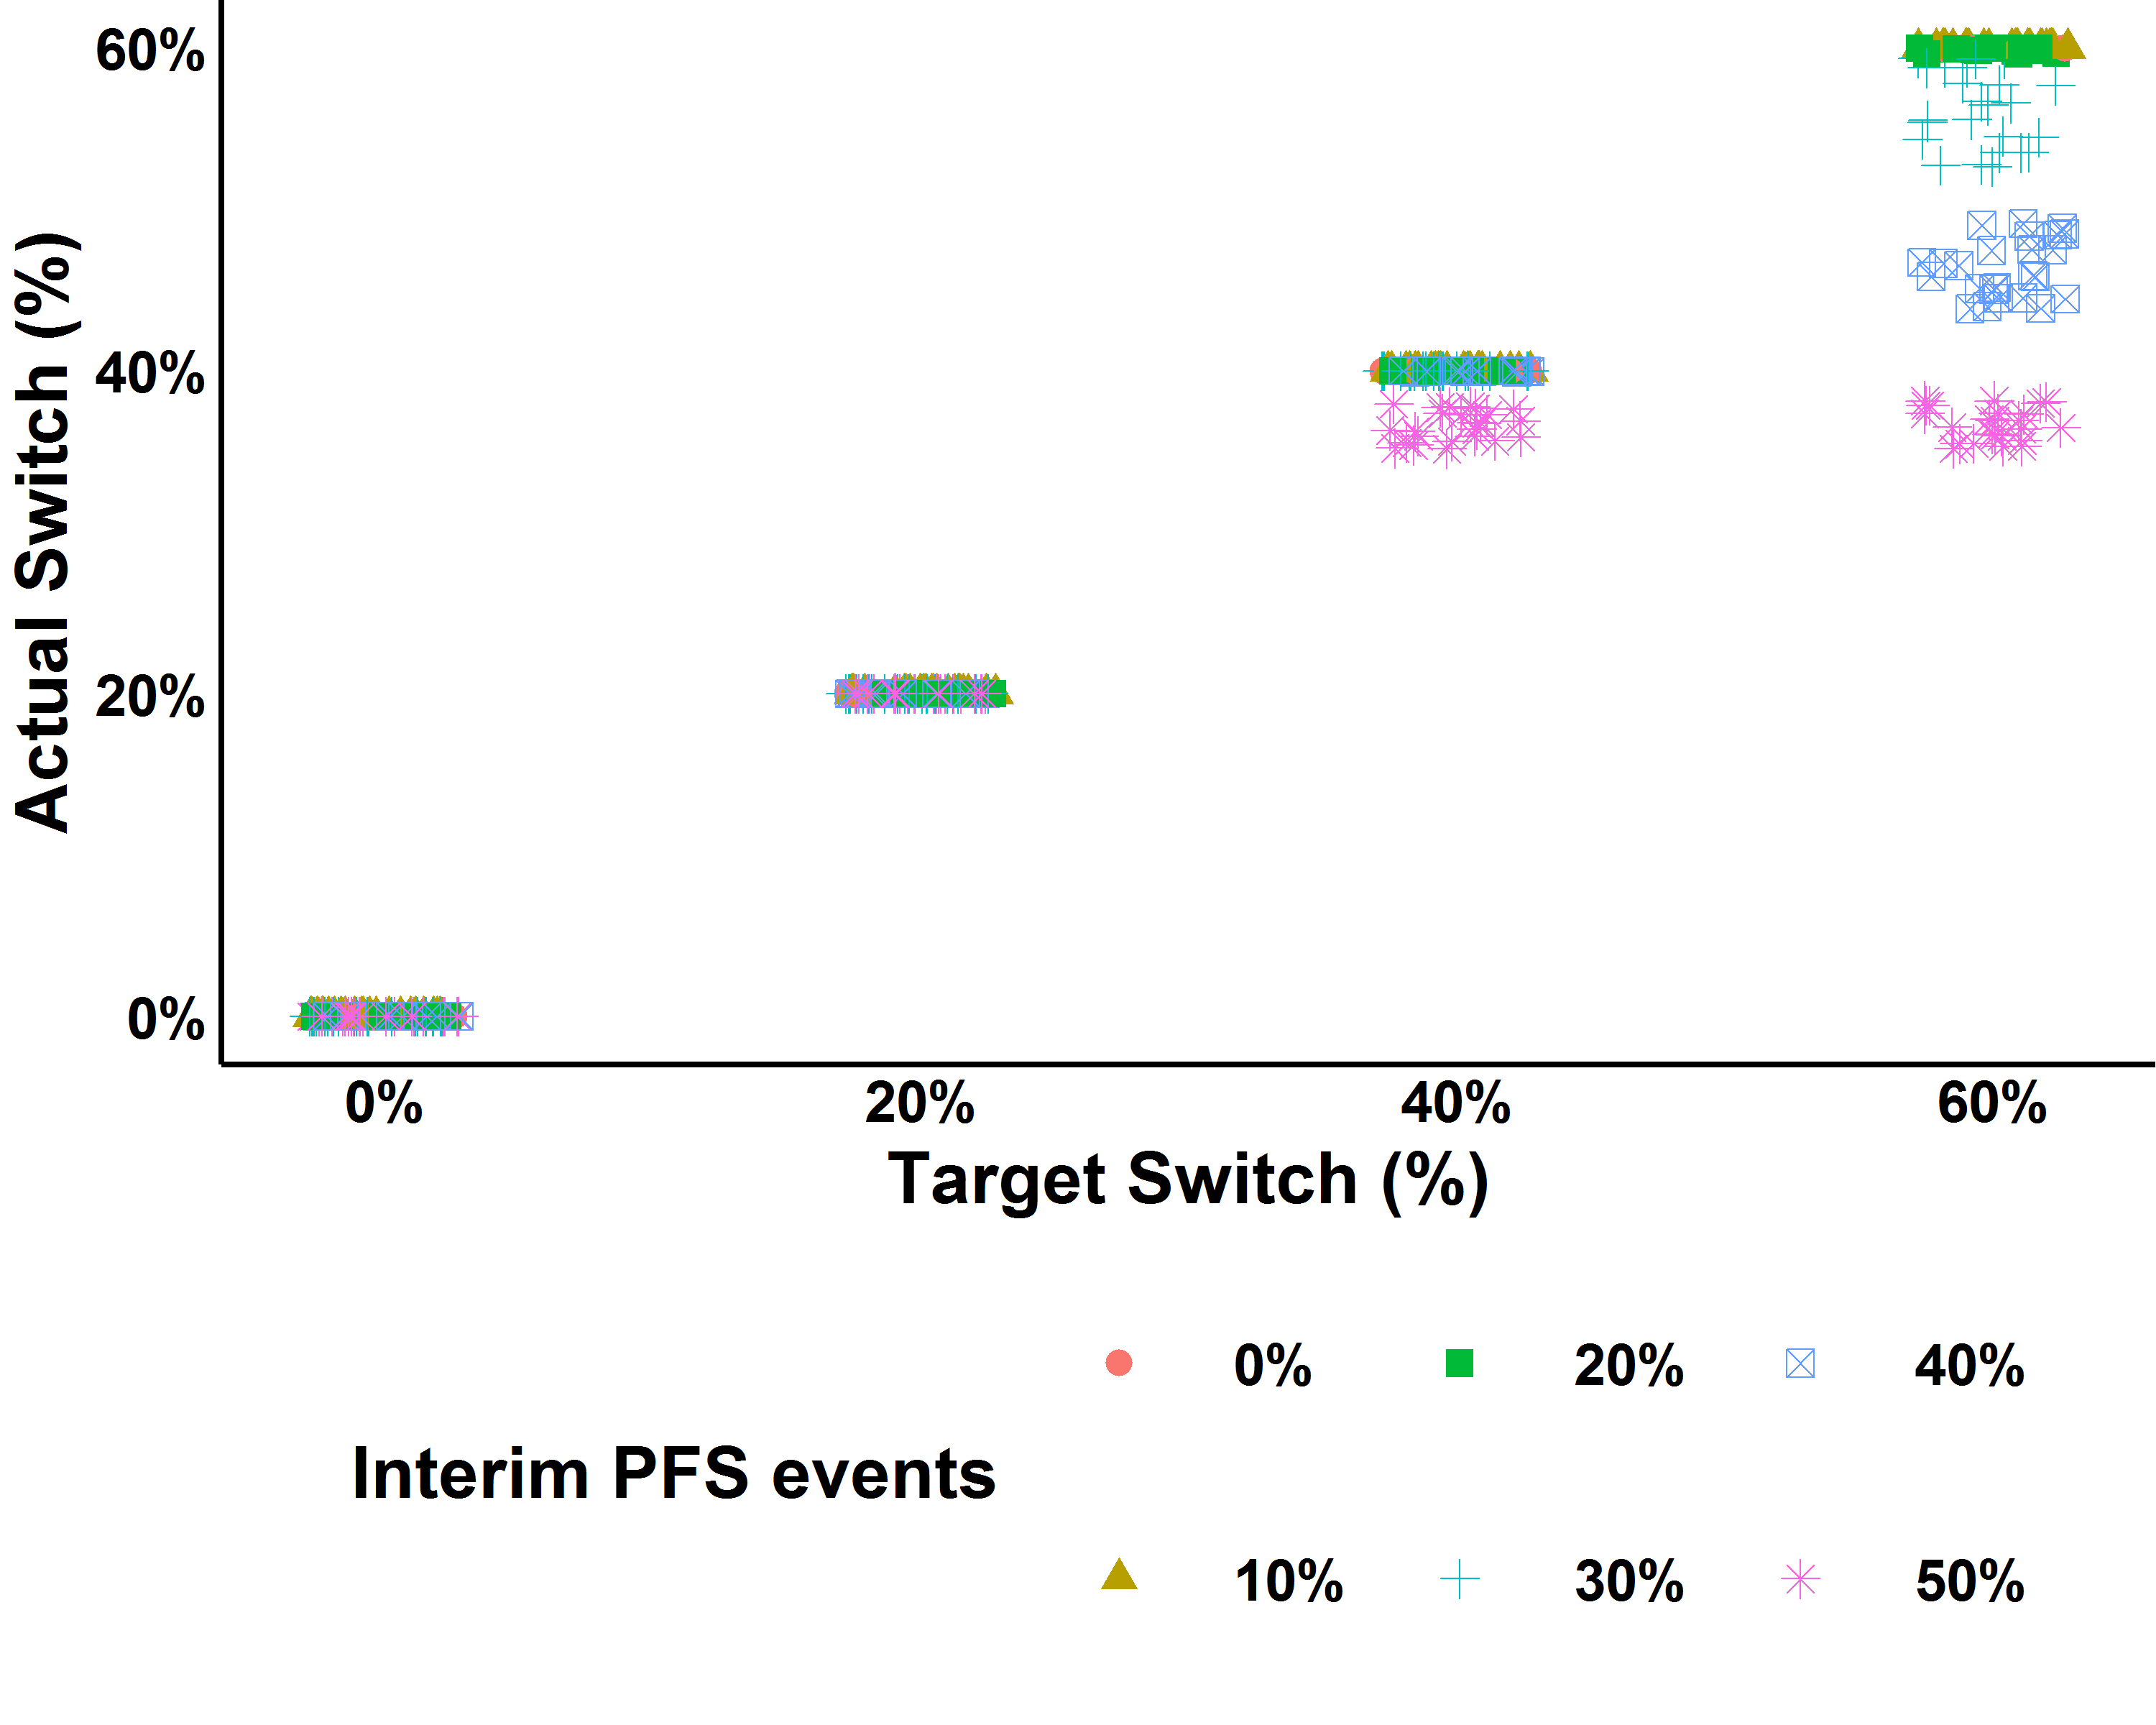
\includegraphics[width=10cm]{images/chap_simdesign/p_switch.png}
\caption{\label{F:chap_sim_design:pswitch} Figure illustrating the relationship between the percent of progression free survival events required at the interim analysis where switch is allowed and the resulting amount of switching relative to the target amount. It can be seen that by delaying switch until after an interim occurs the actual proportion of control arm patients who switch can be considerably reduced. Due to this interaction for the simulation studies described in Chapter \ref{C:chap_sim2} and Chapter \ref{C:chap_sim3} only the proportion of patients who switch will be varied. That is the interim PFS events prior to switch will be always set at 0\%.}
\end{figure}






